\chapterimage{SolidsStabilizationDigestion.png} % Chapter heading image

\chapter{Solids Stabilization - Digestion}


\begin{itemize}
                \item Sludge digestion is a microbiological process to treat - stabilize, the wastewater solids
                \item As part of digestion, the organic material present is biodegraded by microorganisms.  It is the most common sludge stabilization method.  
                \item There are two major sludge digestion processes - aerobic digestion which utilizes aerobic microorganisms and anaerobic digestion which utilizes anaerobic microorganisms.\\
            \end{itemize}
        \begin{center} Comparison of aerobic and anaerobic digestion:
        \setlength{\arrayrulewidth}{0.2mm}
\setlength{\tabcolsep}{8 pt}
\renewcommand{\arraystretch}{0.6}
        \begin{tabular}{| c| p{10.5cm}|}\hline

        \small Methane production (fuel use potential)& \small Unlike anaerobic digestion, aerobic digestion does not produce methane\\
        \hline

        \small Energy consumption & \small Aerobic digestion has higher energy needs as air supply is required to support the aerobic activity.  The energy needs for an anaerobic digester is limited to mixing the digester and maintaining digester temperatures\\
        \hline

        \small Biomass production & \small Anaerobic digestion produces only about 20\% of the biomass produced by aerobic digestion\\
        \hline

        \small Dewaterability of sludge produced & Compared to anaerobic digestion, aerobic digestion produces sludge with poor dewaterability which leads to producing cake with lower solids content and therefore more expensive to haul\\
        \hline

        \small Ammonia concentration & Siginifcant ammonia is produced as part of anaerobic digestion which imposes additional ammonia removal needs particularly for plants with nitrogen discharge thresholds\\
        \hline

        \small Sludge odors & Aerobic digestion has much less odor issues compared to anerobic digestion \\
        \hline

        \small Capital cost & Initial capital costs are higher for anaerobic digesters due to higher SRT requirements is higher - methanogens are slower growing\\
        \hline

        \small Weather impacts & \small Process efficiency of aerobic digester drops in cold weather.  The anerobic digestion is not affected by weather as the sludge in the digester is maintained at the desired temperature \\
        \hline
            \end{tabular}
             \end{center}

        For this class we will focus only on anaerboic digestion - the most common method - as anaerboic digestion generates digester gas which can be used as fuel and also due to its lower energy demands.
\newpage
\section{Digester design}\index{Digester design}
            
            \begin{itemize}
                \item The anaerobic digester is typically a large cylindrical concrete tank
                \item The digester is operated as a continuous process at a fixed volume
                \item As sludge is fed into the digester it displaces an equal amount of sludge which leaves the digester through the digester overflow system - see the digester overflow system design diagram below
                \item The digester overflow system is designed to allow for selecting the level from which the sludge overflows
                \item The sludge typically occupies 70 - 90\% of the total digester volume and the methane carbon dioxide gas mixture occupies the headspace from where it is withdrawn also on a continuous basis.
                \item The digester can be constructed with either a fixed or floating roof.
            \end{itemize}

\begin{figure}[]
	\begin{center}
		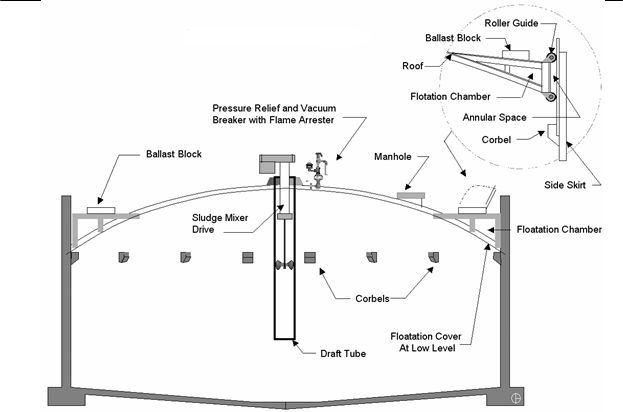
\includegraphics[scale=0.7]{DigesterFloatingCover}\\
			\caption{Floating Dome Anaerobic Digestion}
	\end{center}
	\end{figure}
	
	
\begin{figure}[]
	\begin{center}
		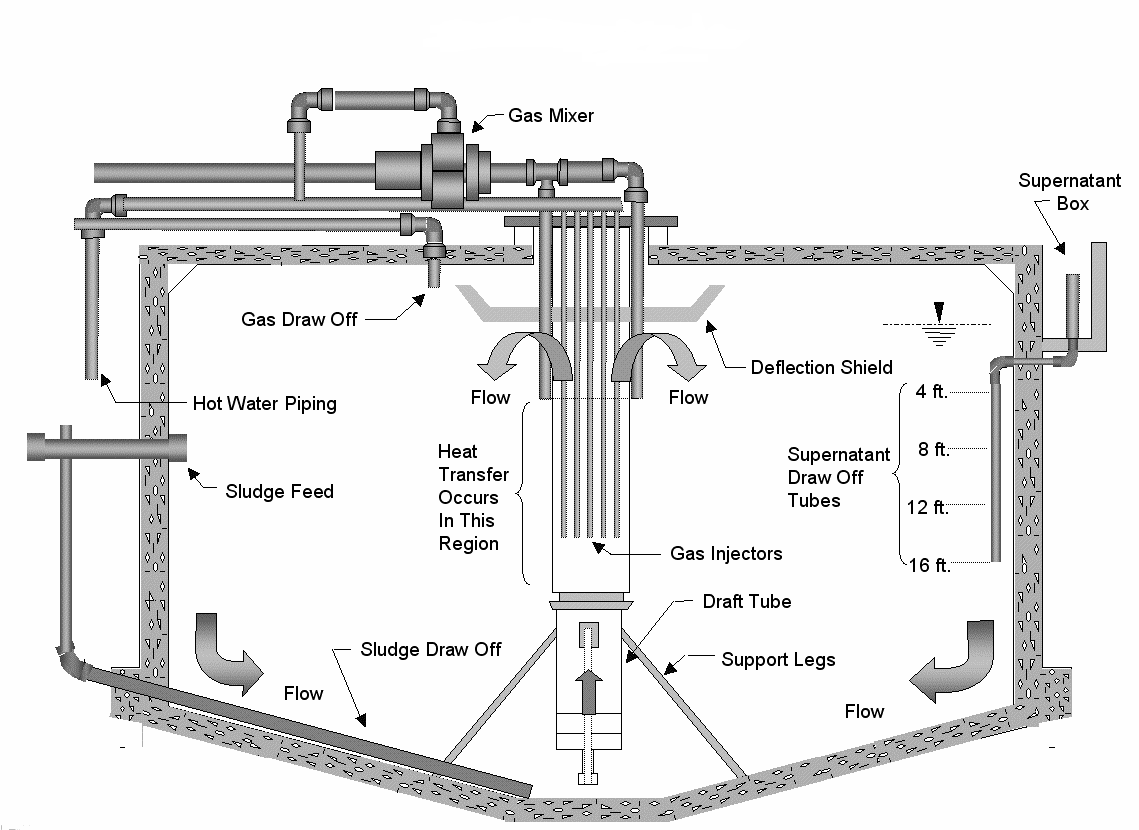
\includegraphics[scale=0.43]{DigesterFixedCover}\\
			\caption{Fixed Dome Anaerobic Digestion}
	\end{center}
	\end{figure}
	
	
\begin{figure}[]
	\begin{center}
		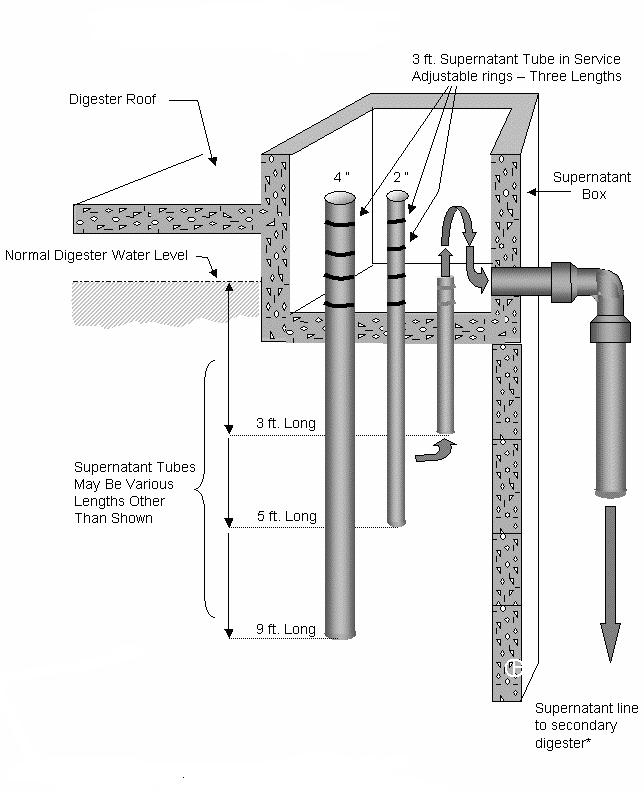
\includegraphics[scale=0.5]{DigesterSupernatantTubes}\\
			\caption{Digestion Overflow System}
	\end{center}
	\end{figure}


\section{Types of anaerobic digestion systems}\index{Types of anaerobic digestion systems}                

\vspace{1cm}
\begin{minipage}{.25\textwidth}
      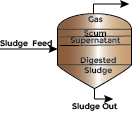
\includegraphics[width=\linewidth, height=45mm]{DigestionLowRate}
    \end{minipage}
\hspace{1cm}
\begin{minipage}{.35\textwidth}
        \end{minipage}
\begin{minipage}{.50\textwidth}\textbf{Low-Rate}\\
$\bullet$ No mixing provided\\
$\bullet$ Long detention time of 30 to 60 days\\
$\bullet$ Suitable for low organic loading\\
$\bullet$ Intermittent sludge feed\\
$\bullet$ Stabilized solids settle to the bottom and are removed periodically\\
$\bullet$ Suitable for small wastewater treatment plants\\ \end{minipage}

\vspace{1cm}

\begin{minipage}{.25\textwidth}

		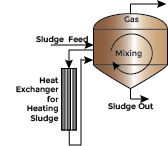
\includegraphics[width=\linewidth, height=45mm]{DigesterHighRate_1}\\
    \end{minipage}
    \hspace{1cm}
\begin{minipage}{.35\textwidth}
        \end{minipage}
\begin{minipage}{.50\textwidth}\textbf{High-Rate}\\
$\bullet$ Mixing and external heating provided\\
$\bullet$ Uniform feeding\\
$\bullet$ Typical detention times of 10 to 20 days\\
$\bullet$ Most common\\  \end{minipage}

\vspace{1cm}

\begin{minipage}{.5\textwidth}

		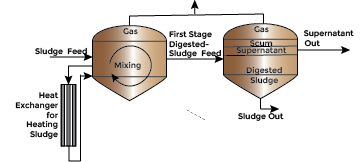
\includegraphics[width=\linewidth, height=45mm]{DigestionTwoStageAnaerobic}\\
    \end{minipage}
\begin{minipage}{.35\textwidth}\textbf{Two-stage}\\
$\bullet$ Digestion occurs in the heated and mixed primary digester vessel\\
$\bullet$ The unheated secondary tank serves as storage for digested solids and as a source of seed\\  \end{minipage}\\
\vspace{1cm}

\vspace{1cm}

\setlength{\arrayrulewidth}{0.1mm}
\setlength{\tabcolsep}{8 pt}
\renewcommand{\arraystretch}{0.8}
%{\rowcolors{2}{green!60!yellow!50}{green!30!yellow!40}
\begin{tabular}{| p{4cm}| p{6cm}|p{6cm}|}\hline
\multicolumn{3}{|c|}{\textbf{Summary Conditions for Anaerobic Sludge Digestion}} \\ \hline

\small Temperature and detention time & \small Psychrophillic \newline Mesophillic - Normal range  \newline Mesophilic Most common \newline Thermophillic & \small 50 - 65 F 50 - 180 days \newline 68 - 113 F \newline 95 - 98 F 15 - 30 days \newline 113 - 135 F 5 - 12 days\\

\small pH & \small Optimal \newline General Range & \small 7.0 to 7.1 \newline 6.4 to 7.4\\

\small VS loading rate (high rate digester) & \small Optimal & 0.1 and 0.2 lbs VS/day/ ft$^3$\\

\small Gas production & \small Per pound volatile solids added \newline Per pound volatile solids destroyed & \small 8-12 cu. ft \newline 16-18 cu. ft.\\
\hline

\small Gas Composition & \small Methane \newline Carbon dioxide \newline Hydrogen sulfide  & \small 65\% \newline 35\% \newline Trace\\
\hline

\small Volatile acid concentration (as acetic acid) & \small Normal \newline Maximum  & \small 200-800 mg/L \newline 2000 mg/L\\
\hline

\small Alkalinity Concentration  & \small Normal & \small 2,000-3,500 mg/L (as calcium carbonate) \newline
3,000-5,000 mg/L (as bicarbonate)\\
\hline

\small Volatile acids to alkalinity ratio & \small Desirable \newline Upset condition & \small $<0.25$ \newline $>0.4$ \\
\hline

	\end{tabular}\\


\section{Digestion parameters and control}\index{Digestion parameters and control}

\subsection{Digestion temperature}\index{Digestion temperature}
                    \begin{itemize}
                        \item The anaerobic digestion is temperature sensitive and temperature of the sludge in the digester needs to be controlled to ensure proper operation.
                        \item The activity and type of bacteria present in the digester is dictated by the operating temperature of the digester.
                        \item Anaerobic digestion can be in the following three temperature ranges, each of which has its own unique microbiology.\\
                            \begin{enumerate}[i.]
                            \definecolor{shadecolor}{RGB}{225, 235, 235}
                          
                                \begin{snugshade*}
                                \item \noindent\textsc{Psychrophilic digestion}
                                \end{snugshade*}
                                If operating in this temperature regime, the digesters are maintained between 50  - 65 F.  This regimen is not commonly used.  Digestion in this range requires 50 to 180 days depending on the target volatile matter reduction\\

                                \begin{snugshade*}
                                \item \noindent\textsc{Mesophilic digestion:}
                                \end{snugshade*}
                                These digesters operate between 68  - 113 F.  Most common operating temperatures for mesophilic digesters is between 95 – 98 F and the typical number of days required for digestion is between 15 to 30 days.\\
                                
                                \begin{snugshade*}
                                \item \noindent\textsc{Thermohillic digestion:}
                                \end{snugshade*}
                                These digesters’ optimal operating temperatures range is between 113 -  135 F and it typically requires 5 to 12 days.\\
                            \end{enumerate}
                        \item A digester does not tolerate temperature fluctuations and need to be maintained at stable temperatures for a significant duration.  
                        \item As a rule of thumb temperature of a digester should not be changed more than 1 per day.
                        \item Temperature fluctuations will destroy the microbiological balance leading to digester failure.
                        \item External heating is provided to maintain sludge temperatures in the digester.
                        \item Temperature fluctuations also can be minimized by feeding the system at frequent intervals.\\
                        \item An external or internal heat exchanger or direct steam injection is typically used for maintaining the sludge temperature
                    \end{itemize}

\subsection{Digestion mixing}\index{Digestion mixing}
            
                    A sludge mixing system is integral to the digester design.  It performs three main functions:  
                        \begin{enumerate}[1.]
                            \item It allows for the bacteria to properly come in contact with the food.  
                            \item It prevents accumulation of grit and scum in the digester which could lead to dead zones.
                            \item It allows for maintaining uniform temperature.  Typical mixing system designs achieve a turnover time of 30 to 45 minutes.
                        \end{enumerate}

\subsection{Digestion feed}\index{Digestion feed}
                    \begin{itemize}
                        \item The sludge feed to the digester has a total solids content of about 3 – 6\%.  
                        \item 70\% of the total solids fed are organic solids.  
                        \item These organic solids are measured as volatile solids (VS)
                        \item Hydraulic or Sludge retention time (SRT) is calculated by dividing the digester volume by the daily sludge flow
                        $$Digester \enspace SRT \enspace (days) =\dfrac{Digester \enspace Volume \enspace (ft^3 \enspace or \enspace gallons)}{Sludge \enspace Feed \enspace (ft^3 \enspace or \enspace gallons \enspace per \enspace day)}$$
                        \item The SRT in an anaerobic digester typically ranges from 10 to 20 days.
                        \item A minimum SRT is essential to the digestion process to ensure that the necessary microorganisms are being produced at the same rate as they are removed from the system each day  \\
                        \item Accumulation of grit in the bottom or scum at the top of the digester would effectively reduce the working volume of the digester
                        \item The amount of digester influent being pumped and the percent VS of the waste are a measure of the digester’s organic loading rate (influent mass per time)
                        \item Control of the amount of volatile solids loading is one of the key critical operational control parameter. 
                        \item Volatile solids loading rate of the digester is the mass of VS added to the digester each day divided by the operating volume of the digester – lbs VS/day/ft$^3$
                        \item Typical high rate digesters VS loading range between 0.1 and 0.2 lbs VS/day/ ft$^3$
                        \item The rate of digestion depends on the type of organic material present.  
                        \item The constituents of the organic material in primary sludge is typically feces, and plant and animal origin material.  This organic material is relatively easy to digest compared to the organics in the secondary sludge which is primarily living and dead microorganisms and metabolic byproducts associated with microbiological growth and decay.
                        \item Typical primary sludge from a treatment plant with preliminary treatment contains approximately 65\% organic material.  80\% of this organic material is typically destroyed in the digester.  Whereas, the secondary sludge typically contains 90\% organics and only 60\% of the secondary sludge organics is destroyed.
                    \end{itemize}

\subsection{Volatile solids breakdown}\index{Volatile solids breakdown}
                        \begin{itemize}
                            \item The volatile solids content of the sludge entering and leaving the digester are measured to quantify the solids removal in the digester
                            \item The expected reduction of volatile solids of a properly operating digester is 40-60\% of the total volatile solids present in raw sludge feed.
                            \item The volatile solids in the feed sludge would be about 70\% to 75\% while the digested sludge would be 45\% to 50\% volatile solids
                            \item The expected reduction of volatile solids of a properly operating digester is 40-60\% of the total volatile solids present in raw sludge feed
                            \item The volatile solids reduction of the digester is provided by the Van Kleeck equation 
                            $$Digester \enspace VS \enspace reduction (\%)=\dfrac{VS_{in}-VS_{out}}{VS_{in}-VS_{in}*VS_{out}}*100$$
                            \item Digester volatile solids concentration is typically expressed as a percentage of the sludge total solids
                            \item 70\% VS which means that 70\% of the total solids is volatile solids
                            \item The value of $VS_{in}$ and $VS_{out}$ for the digester VS reduction (Van Kleek) equation above should be in fraction and not as a percentage.
                            \item For example:  for a 70\% VS content use 0.7 in the equation.  Likewise 0.525 is used for 52.5\% VS concentration\\
                            \item Higher volatile solids reduction implies higher gas production and lower biosolids hauling costs
                            \item Breakdown of volatile matter in the sludge ultimately into methane (CH$_4$) and carbon dioxide (CO$_2$) occurs in multiple steps involving different groups of microorganisms.\\
                            Step 1. This is the hydrolysis step where the complex organic matter in the sludge including carbohydrates, proteins, lignin, and lipids are converted to simpler compounds including sugars, soluble fatty acids and amines.\\
                            Step 2. This involves formation of volatile acids from the products from Step 1.  This is the acid formation step.\\
                            Step 3. The acid formed in Step 2 is converted into methane and carbon dioxide.  This step is accomplished by a group of methane forming bacteria.\\
                            \item The digester conditions are maintained to ensure optimal conditions conducive to the activity of the methane formers.Good digester operations requires ensuring that conditions are kept favorable for the methane formers
                        \end{itemize}
     
\subsection{Digester pH and alkalinity}\index{Digester pH and alkalinity}
                    \begin{itemize}
                        \item The anaerobic digestion requires a symbiotic relationship between the different groups of microorganisms involved. 
                        \item Each group of organisms involved in the anaerobic digestion process have an optimal pH for maximum rate of reaction – \\
                        Hydrolysis: pH 5-7 optimal\\ 
                        Acid formation: pH 5-7 optimal – \\
                        Methane formation: pH 7-8 optimal, pH 6.5-8.5 operational\\
                        \item In a healthy digester the volatile acids produced in Step 2 are used in Step 3 as food by the methane formers at about the same rate as they are produced.  
                        \item As the methane forming microorganisms in the digesters are very sensitive to the digester conditions including organic content, pH, temperature and toxins and also grow very slowly, it is necessary to maintain the digester pH close to neutral
                        \item The conversion of the volatile fatty acids to methane by methane formers allow for controlling the accumulation of volatile acids
                        \item If the activity of methane formers is suppressed due to conditions such as low pH, volatile acids will accumulate potentially causing the digester to become "sour"
                        \item In a normally operating digester, the alkalinity present in the sludge prevents the pH from dropping due to the formation of volatile acids during Step 2.
                        \item The alkalinity consumed due to the acids formed in Step 2 is replenished in Step 3 by the formation of bicarbonate from the CO$_2$ and ammonia produced during digestion.\\
                        $$NH_3+H_2O+CO_2 \to NH_4HCO_3$$  
                         \item Unlike the acid formers,   Thus, if the digester condition such as the pH was to change – drop because of the formation of acids and a lack of alkalinity, Step 3 will not happen resulting in the digester pH dropping even further resulting in a “sour” digester condition.
                        \item When acid formers out produce the methane formers the volatile acids increase sharply
                        \item The methane formers are the key to digester operation and are very vulnerable to low pH There needs to be sufficient alkalinity present to prevent pH changes as the volatile fatty acids are being formed.
                        \item If sufficient alkalinity is not present the pH will drop further inhibiting the activity of methane formers and the digester will turn “sour”
                        \item The bicarbonate ion (HCO$_3^-$ ) is the main source of buffering capacity to maintain the system’s pH in the range of 6.5 – 7.6. The concentration of HCO$_3^-$  in solution is related to the percent of carbon dioxide in the gas phase 
                        \item Alkalinity consumed by the acid production is offset by alkalinity produced as part of the methanogenic activity
                        \item Regular monitoring the digester alkalinity and volatile acids is vital in ensuring a stable digestion process.
                        \item In a well operating digester the volatile acids expressed as acetic acid would be in the range of 50 to 500 mg/L and the alkalinity expressed as calcium carbonate would be in the range of 2,000 to 3,000 mg/L (bicarbonate alkalinity of 2,500mg/L and 5,000mg/L)
                        \item The volatile acid-to-alkalinity ratio indicates if the digester has enough buffering capacity for the volatile acids being produced.
                         \item Increase in volatile acid to-alkalinity ratio will increase the potential for pH decrease which would result in an upset digester.
                         \item In general keeping the volatile acids to alkalinity ratio at 0.25 or less is desirable for good operations.
                        \item Ratios above 0.4 indicate upset and the need for corrective action.\\
                                            \end{itemize}
\subsection{Digester pH control}\index{Digester pH control}                        
    
                            \begin{itemize}
                                \item Following chemicals: calcium oxide, calcium hydroxide, anhydrous ammonia, Ammonia (liquid), ammonium hydroxide, sodium carbonate, sodium bicarbonate, and sodium hydroxide have been used for increasing the pH of a sour digester.
                                \item The use of calcium oxide (quicklime) or calcium hydroxide (slaked or hydrated lime) is probably the most dangerous if mixed with water prior to feeding.   If instead of adding these two chemicals to water for digester feeding, adding water to these chemicals would pose the threat of a violent reaction and splattering of this strong caustic.\\ 

                                Excess lime should be avoided as lime reacts with carbon dioxide to form calcium carbonate.

                                $Ca(OH)_2 + CO_2 \rightarrow CaCO_3 + H_2O$ 

                                If carbon dioxide is removed too rapidly or in too large a quantity from the sludge, then carbon dioxide from the biogas will replace the carbon dioxide lost from the sludge. When carbon dioxide is lost from the biogas, a partial vacuum condition develops under the digester dome. This condition may cause the digester cover to collapse. Also, as the concentration of alkalinity increases in the anaerobic digester, the continued use of quick lime results in the precipitation of calcium carbonate.

                                \item Sodium hydroxide would be the next most dangerous followed by ammonium hydroxide.  
                                \item The use of anhydrous ammonia should be limited to facilities that have the equipment to handle gas cylinders and that have feed connections or the ability to make the necessary feed connections.
                                \item The feeding of lime can only raise the digester pH to about 6.8. When lime is added it reacts with carbon dioxide to form calcium bicarbonate. Excessive feeding of lime causes insoluble calcium carbonate to form. In addition excessive lime may remove too much carbon dioxide which could lower gas pressures or even the formation of a vacuum. This could cause air to be drawn into the digester and cause an explosive gas mixture.
                            \end{itemize}
                

\subsection{Digester gas production}\index{Digester gas production} 

                    \begin{itemize}
                        \item In the anaerobic digestion process microorganisms convert volatile matter into mainly methane (CH$_4$) and carbon dioxide (CO$_2$)
                        \item Typical composition of digester gas is about 58 - 65\% methane and 30 - 35\% CO2 it also includes traces of ammonia nitrogen, hydrogen sulfide, and other gases.
                        \item Monitoring digester gas production is one of the more important operational parameter.  
                        \item Gas production ranges between 10 to 16 cubic feet per pound of volatile matter destroyed and the gas production remains stable over time.
                        \item Low gas production is an indicator of digester issue related to - toxicity, temperature, volatile acid to alkalinity ratio, mixing, or feed rates.
                    \end{itemize}

\subsection{Digester failure}\index{Digester failure}   

                    \begin{itemize}
                        \item Digester failure conditions are marked by conditions which include increases in:
                        \begin{itemize}
                            \item volatile acids
                            \item volatile acids: alkalinity ratio
                            \item drop in pH
                            \item drop in gas production, and 
                            \item an increase in $CO_2$ concentration
                        \end{itemize}
                        \item The failure is typically attributable to factors including overloading, toxicity and temperature control issues.
                        \item Digester failure can be controlled by:
                        \begin{itemize}
                            \item stopping or reducing the sludge feed
                            \item exercising pH controls by adding alkaline chemicals, and 
                            \item through reseeding the digester with sludge from another healthy digester
                        \end{itemize}
                    \end{itemize}
\subsection{Digester toxicity issues}\index{Digester toxicity issues} 

                \begin{itemize}
                \item Toxicity could severely impact a digester performance.
                \item Contributors to toxicity issues include high concentrations of ammonia and toxic metals such as arsenic, cadmium, chromium (hexavalent), copper, nickel, zinc. 
                \item Ammonia toxicity: Ammonia from industrial sources, organic overloading, or from using anhydrous ammonia to correct a digester pH problem can cause a die-off of bacteria; ammonia toxicity begins around 1,500 mg/L and is totally toxic at 3,000 mg/L.  
                \end{itemize}

\subsection{Nutrients and trace constituents requirement}\index{Nutrients and trace constituents requirement}
        The major nutrients required for anaerobic digestion are nitrogen and phosphorus. An average cell contains approximately 12.5 percent nitrogen and 2 percent phosphorus. Sodium, potassium, calcium, magnesium, chloride, and sulfate ions are also required for proper digestion.\\

\section{Digester safety}\index{Digester safety}
\begin{enumerate}[A.]
    \item Pressure \& Vacuum Protection:\\
        \begin{itemize}
            \item In a digester,as the gas production and sludge withdrawal is continuous, there exists a potential to create pressurized or vacuum conditions within the digester which could jeopardize the structural integrity of the digester.  
            \item Typically the gas in the digester dome is maintained at a pressure of 8-9 inches of water column.  
            \item A pressure relief valve is designed into the digester dome which allows to protect the digester from excessive pressure or vacuum conditions.  
            \item In the event of the digester dome being under excessive pressure, the valve will open to relieve the pressure and likewise if the valve senses a low pressure or vacuum condition, it will open up just enough to let in the air to bring the gas in the digester dome back to normal, set pressure.
        \end{itemize}
    \item Fire and Explosion Protection:  \\
        \begin{itemize}
            \item For a fire or explosion to occur, following three conditions must be met simultaneously:\\
                \begin{enumerate} 
                    \item Presence of fuel – combustible material
                    \item Oxygen (air) must exist in certain proportions, and
                    \item Ignition source, such as a spark or flame.
                \end{enumerate}  
            \item Digester gas contains methane which is a combustible gas.  
            \item The ratio of fuel and oxygen that is required varies with each combustible gas or vapor. The Lower Explosive Limit (LEL) and (UEL) for methane is 5\% and 15\% respectively.  
            \item A 5\% LEL implies that a methane concentration in air of less than 5\% is too “lean” to burn and a 15\% UEL implies that a concentration of methane exceeding 15\% in air would be too “rich” to burn.  So for methane, the flammable range is between 5\% and 15\%.  As the digester gas methane content is typically between 60 to 65\%, dilution of digester gas with air has the potential to form an explosive mixture. 
            \item A flame arrestor is typically installed at the outlet of the digester gas piping to protect the digester from any external heat or ignition source.  The flame arrestor is essentially a heat exchanger which cools down the ignition source or flame entering the digester. 
        \end{itemize}
        \begin{center}
            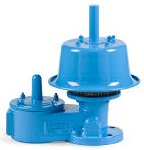
\includegraphics[scale=0.8]{DigesterPressureRelief} \hspace{5cm} 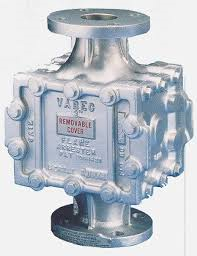
\includegraphics[scale=0.5]{DigesterFlameArrestor} \\
        \end{center}
        \hspace{2cm}\textbf{Digester Pressure Relief} \hspace{3cm} \textbf{Digester Flame Arrestor}\\
\end{enumerate}



\newpage
\section*{Chapter Assessment}
\begin{tcolorbox}[breakable, enhanced,
colframe=blue!25,
colback=blue!10,
coltitle=blue!20!black,  
title= Chapter Assessment]

\begin{enumerate}

\item  A change in the-pH-of digesting sludge in anaerobic digester is the best early warning indicator of potential digester upset. \\

a. True \\
b. False \\

\item  A good maintenance program should be established for all flame arresters to ensure they are all set at the recommended "pop-off' pressures. \\

a. True \\
b. False \\

\item  A healthy anaerobic digester should have a carbon dioxide concentration of more than 40\%. \\

a. True \\
b. False \\

\item  A high rate anaerobic digester is always heated and mixed. \\

a. True
b.False \\

\item  Anaerobically digested sludge produces gas as a by-product. The gas produced is of little or no value. \\

a. True \\
b. False \\

\item  Identify the incorrect statement regarding anaerobic digestion. \\

a. An anaerobic digester with pH of 7.05, an alkalinity of 2,900 mg/l and a volatile acid concentration of 250 mg/l is probably operating normally. \\
b. Sodium bicarbonate may be used in place of lime to neutralize a sour anaerobic digester. \\
c. When adding lime to a sour anaerobic digester, it is important to add an excess of this chemical to act as a reservoir of alkalinity. \\
d. Ferrous sulfate may be added to an anaerobic digester to reduce hydrogen sulfide concentration where air quality is of concern. \\
e. Gas production from anaerobic digester may be expressed as cubic feet of gas produced per pound of volatile matter added per day. \\

\item  One action that may be taken to improve the health of an anaerobic digester that is going sour would be to: \\

a. Add small doses of lime daily to maintain the digester pH above 7.0. \\
b. Add ferrous sulfate to reduce the concentration of hydrogen sulfide in the digester. \\
c. Add seed sludge from a healthy primary digester. \\
d. Pump raw sludge to this digester more frequently so that this sludge has a higher pH. \\
e. Increase the temperature of the digester to favor a population increase of the methane formers. \\

\item  Identify the incorrect statement regarding operation of an anaerobic digester. \\

a. A healthy anaerobic digester would generally have volatile acids in the range of 50 mg/l to 300 mg/l. \\
b. The best strategy for pumping raw sludge to an anaerobic digester is to pump it once or twice a day so that the thickest possible raw sludge may be pumped. \\
c. An anaerobic digester operating at an alkalinity of 3200 mg/l should be able to tolerate a volatile acid concentration of 250 mg/l. \\
d. The change in pH is not a reliable indicator of the changing characteristics of the digesting sludge because the alkalinity in an anaerobic digester acts as a buffer. \\
e. The higher the volatile solid content of the primary sludge being fed to the digester, the higher is the expected volatile reduction. \\

\item  Identify the true statement about anaerobic digesters: \\

a. Carbon dioxide and methane in digester gas should be 65\% and 35\%, respectively. \\
b. Increasing carbon dioxide readings indicate possible organic overload. \\
c. Decreasing mixing will always improve recovery of a sour digester. \\
d. Increasing the frequency and decreasing the amount of sludge pumping will not improve digester performance. \\
e. Reducing the ratio of primary to waste activated sludge will improve gas production. \\

\item  All of the following are normal operating guidelines for a healthy anaerobic digester except for: \\

a. A mesophilic digester operating at 93°F to 98°F. \\
b. Methane gas in the range of approximately 62\% to 70\%. \\
c. Carbon dioxide gas in the range of 30\% to 38\%. \\
d. Organic loading to a high rate digester of 0.15 to 0.2 pounds (Lb) volatile Solids per day per ft3 of digester capacity. \\
e. Bicarbonate alkalinity in the range of 1500 to 1800. \\




\end{enumerate}
\end{tcolorbox}

